
%(BEGIN_QUESTION)
% Copyright 2010, Tony R. Kuphaldt, released under the Creative Commons Attribution License (v 1.0)
% This means you may do almost anything with this work of mine, so long as you give me proper credit

Once upon a time, your instructor was asked to troubleshoot a flow control system where a PLC (Programmable Logic Controller) received a flow measurement signal from a 4-20 mA flow transmitter and sent a 4-20 mA command signal to a variable-frequency motor drive (VFD) turning a pump.  The PLC's job was to turn the pump at the speed necessary to deliver a flow rate at a specified setpoint value:

$$\includegraphics[width=15.5cm]{i04406x01.eps}$$

The operator pressed the ``Start'' button, but the pump refused to turn.  Upon examining the PLC's live program, it was found that the analog input value (a 16 bit binary number) was \$FFFF.  The measured current signal from the flow transmitter was 3.99 mA: just a little bit below 0\% of range, which was reasonable for a no-flow condition.

Your instructor was able to fix this problem by adjusting the ``zero'' screw on the flow transmitter until it output a current signal of exactly 4.00 mA at zero flow.  As soon as this was done, the analog input in the PLC's program registered a value of \$0000, and the pump started up as it was supposed to when the operator pressed the ``Start'' button. 

\vskip 10pt

Explain why this simple transmitter calibration adjustment was able to allow the system to run again, and why the real problem was a design flaw in the PLC.

Hint: The key to understanding what the problem was in this system is the difference between signed and unsigned integers, and how an under-ranged ADC circuit can ``underflow.''

\underbar{file i04406}
%(END_QUESTION)





%(BEGIN_ANSWER)

\noindent
{\bf Partial answer:}

\vskip 10pt

The ADC circuit was designed to output a {\it signed} 16-bit integer value where 4.00 mA would be converted into a value of 0000h and 20.00 mA would be converted into a value of FFFFh.  The control instructions running in the PLC program, meanwhile, interpreted this count value as an {\it unsigned} 16-bit binary quantity.  The problem didn't reveal itself until the fateful day when the flow transmitter's calibration drifted enough to make the current signal 3.99 mA at zero flow rather than 4.00 mA at zero flow.  Recognizing the way the ADC inside the analog input card interpreted this 3.99 mA signal is the key to understanding why the system failed.

\vskip 10pt

Follow-up question: explain why it would be prudent to adjust the flow transmitter's zero slightly higher than 4.00 mA at zero flow to help avoid this problem in the future.

%(END_ANSWER)





%(BEGIN_NOTES)

FFFFh (signed) means a value of $-1$, which is what the ADC output when it ``underflowed'' from the current signal being slightly below 4 mA.  However, that same 16-bit value of FFFFh means +65535 when interpreted as an unsigned value, which would mean absolute top-of-scale (100\%+) for flow.  

The PLC's programming therefore interpreted the underflowed ADC's output as a full-scale flow measurement, and therefore thought it needed to slow the pump (to a standstill) to bring the flow rate {\it down} to setpoint!

%INDEX% Electronics review: ADC resolution

%(END_NOTES)

